\section{Background}
\label{sec:background}

We first explain the most important concepts needed to understand the
algorithms that are proposed in this paper. We first describe \emph{Markov
decision processes (MDPs)}, then  MCTS, then options and finally the \emph{video
game description language (VGDL)}.

\subsection{Markov Decision Processes}
\label{subsec:mdps}
We treat games as MDPs, which provide a mathematical framework for use in
decision making problems. An MDP is a tuple $\langle S, A, T, R \rangle$, where
$S$ denotes the set of states, $A$ is the set of possible actions, $T$ is the
transition function and $R$ is the reward function. Since an MDP is fully
observable, a state in $S$ contains all the information of the game's current
condition: locations of sprites like monsters and portals; the location,
direction and speed of the avatar; which resources the avatar has picked up;
etcetera. $A$ is a finite set of actions, the input an agent can deliver to the
game. $T$ is a transition function defined as $T : S \times A \times S
\rightarrow \left[0,1\right]$; it specifies the probabilities over the possible
next states, when taking an action in a state.  $R$ is a reward function defined
as $R: S \times A \times S \rightarrow \mathbb{R}$. When the game score changes,
the difference is viewed as the reward.  Algorithms maximize the cumulative
reward. In the scope of this paper algorithms only observe state transitions
and rewards when the happen and do not have access to $T$ and $R$.

\subsection{Monte Carlo Tree Search}
\begin{figure}
	\centering
	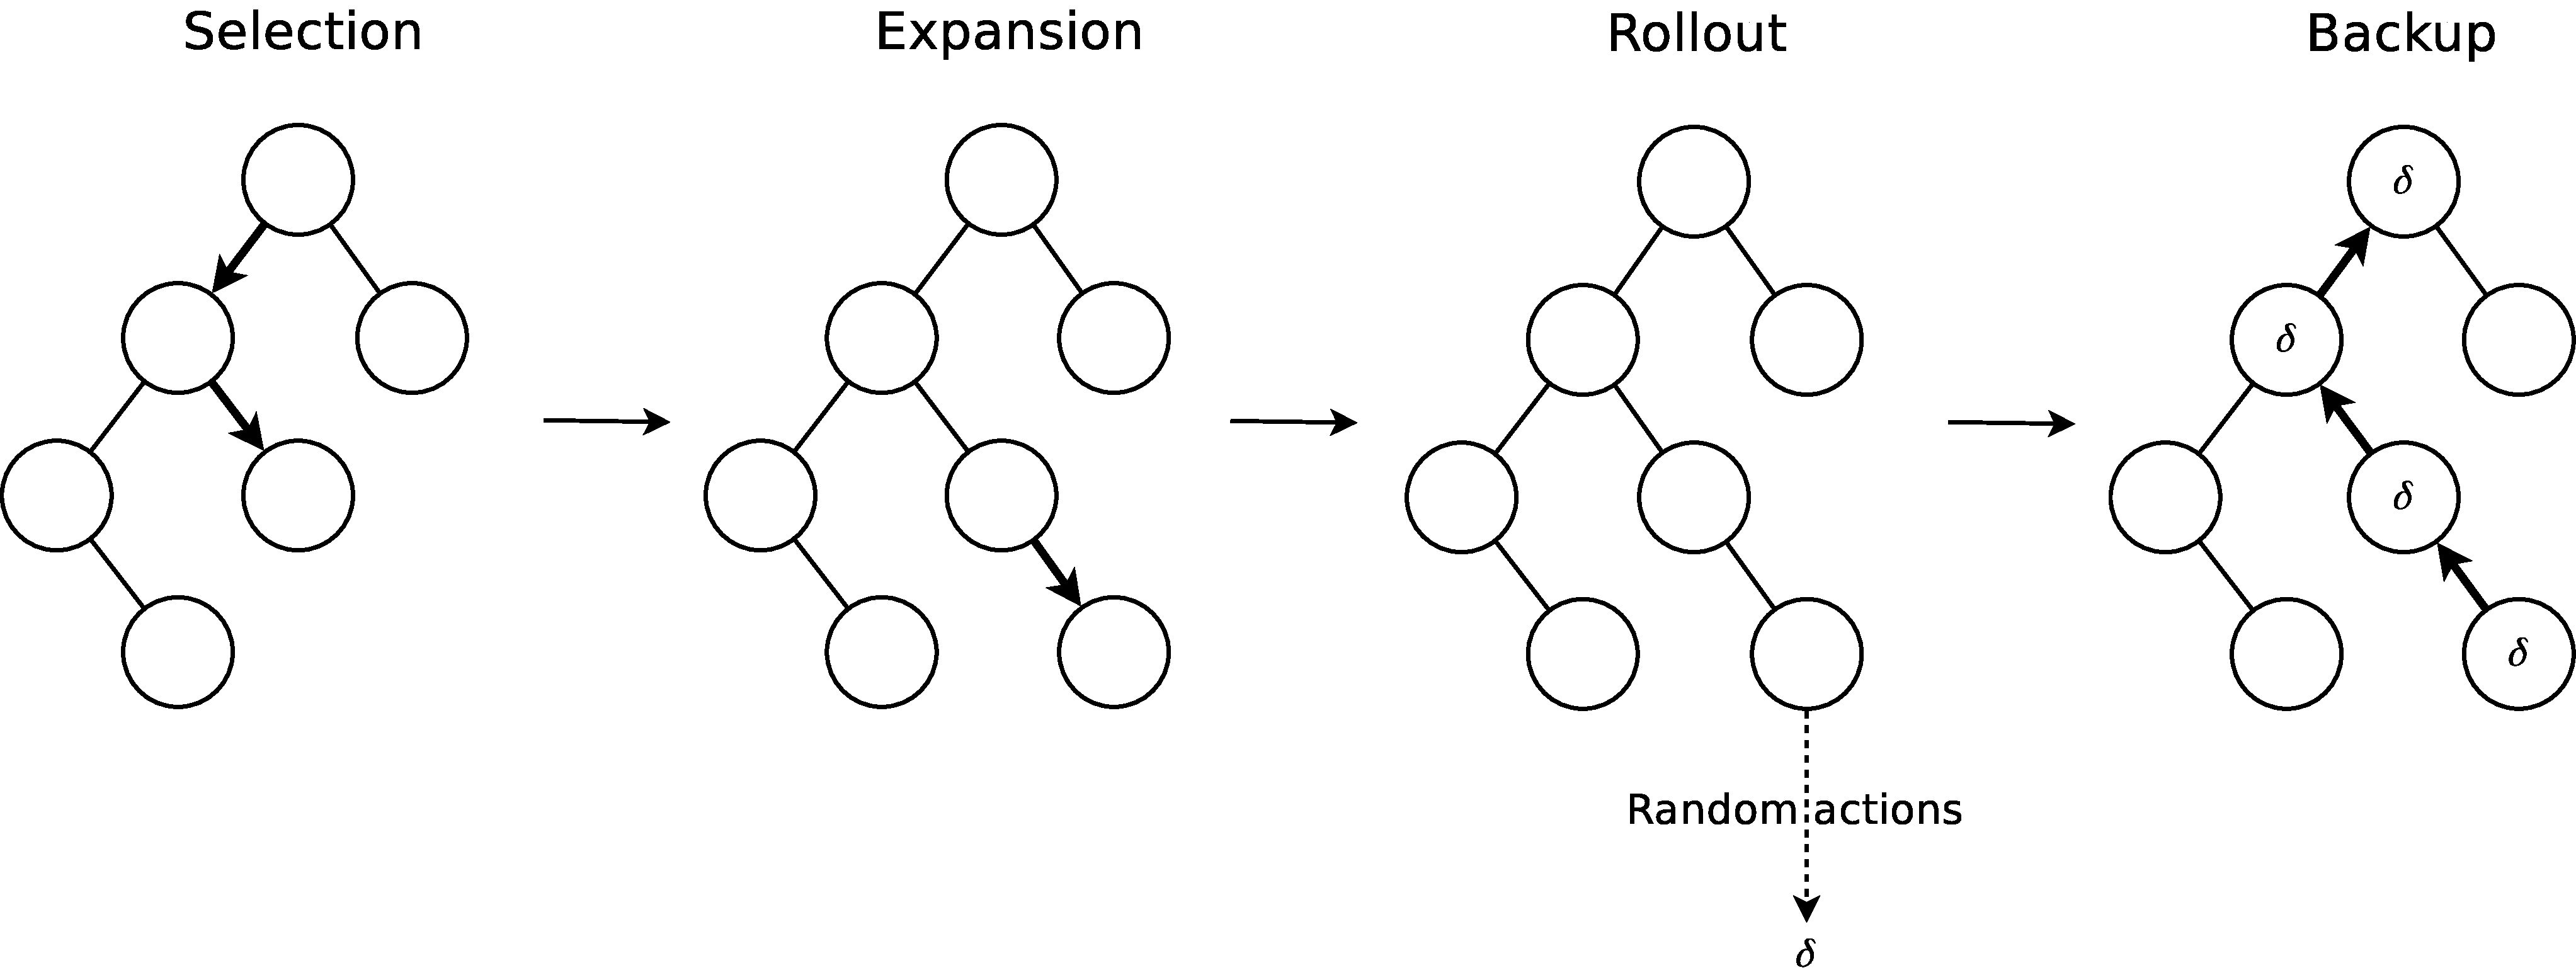
\includegraphics[width=\columnwidth]{includes/mcts-wide-eps-converted-to}
	\caption{One MCTS iteration. This process is repeated in order to improve
	the estimates of action values.}
\label{fig:mcts}
\end{figure}

\label{subsec:mcts}
%Monte Carlo methods have their roots in statistical physics, where they have
%been used to approximate intractable integrals. 
%Abrahamson~\cite{abramson1990expected} demonstrated theoretically that this sampling method might be
%useful for action selection in games as well.  In 2001, Monte Carlo methods were
%effectively used for bridge~\cite{ginsberg2001gib}. 
The success of MCTS started in 2006, when the tree search method and UCT formula
were introduced, yielding good results in Computer
Go~\cite{gelly2006modification}. Since 2006, the algorithm has been extended
with many variations. It is still being used for other computer
games~\cite{browne2012survey}, including the GVGAI
competition~\cite{perez2014knowledge}. In this paper, we use MCTS as the basis
for the new algorithms.

This section explains how MCTS approximates action values for states.  A tree is
built incrementally from the states and actions that are visited in a game. Each
node in the tree represents a state and each edge represents an action taken in
that state. MCTS consists of four phases that are constantly repeated, as
depicted in Figure~\ref{fig:mcts}. The root node of the tree represents the
current game state, Then, the first action is chosen by an \emph{expansion}
strategy and subsequently simulated. This results in a new game state, for which
a node is created.  After expansion, a \emph{rollout} is done from the new node,
which means that a simulation is run from that node, applying random actions
until a predefined stop criterion is met. Finally, the score difference
resulting from the rollout is \emph{backed up} to the root node, which means
that the reward is saved to all visited nodes, after which a new iteration
starts.  When all actions are expanded in a node, that node is deemed
\emph{fully expanded}.  This means that MCTS will use its \emph{selection}
strategy to select child nodes until a node is selected that is not fully
expanded.  Then, the expansion strategy is used to create a new node, after
which a rollout takes place and the results are backed up.

The selection strategy selects optimal actions in internal tree nodes by
analyzing the values of their child nodes. An effective selection
strategy is UCT, which employs an exploration bonus to balance the choice
between poorly explored actions with a high uncertainty about their value and
actions that have been explored extensively, but have a higher
value~\cite{kocsis2006bandit}.  A child node $j$ is selected to maximize
\begin{equation} \label{eq:uct} UCT = v_{s'} + C_p \sqrt{\frac{2 \ln
n_s}{n_{s'}}} \end{equation} Where $v_{s'}$ is the value of child $s'$ as
calculated by the backup function, $n_s$ and $n_{s'}$ are the number of times
nodes $s$ and child $s'$ have been visited and $C_p > 0$ is a constant that
shifts priority from exploration to exploitation.

The traditional expansion strategy is to explore each action at least once in
each node. After all actions have been expanded, the node applies the selection
strategy. Some variants of MCTS reduce the branching
factor of the tree by only expanding the nodes selected by a special expansion
strategy. A specific example is the \emph{crazy stone} algorithm
\cite{coulom2007efficient}, which is an expansion strategy that was originally
designed for Go. We will use an adaptation of this strategy in the algorithm
proposed in Section~\ref{sec:learning}.  When using crazy stone, an action $i$
is selected with a probability proportional to $u_i$ \begin{equation}
\label{eq:crazystone} u_i = \exp\left(K \frac{\mu_0 -
\mu_i}{\sqrt{2\left(\sigma_0^2 + \sigma_i^2\right)}}\right) + \varepsilon_i
\end{equation} Each action has an estimated value $\mu_i$ ordered in such a way
that $\mu_0 > \mu_1 > \cdots > \mu_N$, and a variance $\sigma_i^2$. K is a
constant that influences the exploration --- exploitation trade off.
$\varepsilon_i$ prevents the probability of selecting a move to reach zero. Its
value is proportional to the ordering of the expected values of the possible
actions: $\varepsilon_i = \frac{0.1 + 2^{-i} + a_i}{N}$\@.  Here, $a_i$ is 1
when an action is \emph{an atari move}, a go-specific move that can otherwise
easily be underestimated by MCTS, and otherwise 0.

After a rollout, the reward is backed up, which means that the estimated value
for every node that has been visited in this iteration is updated with the
reward of this simulation. 
%Usually the estimated value of a node is the average
%of all rewards backed up to that node.

\subsection{Options}
\label{subsec:options}

In order to mimic human game playing strategies, such as defining subgoals and
subtasks, we use options. Options, or macro-actions, have been proposed by
Sutton et al.~\cite{sutton1999between} as a method to incorporate temporal
abstraction in reinforcement learning. The majority of the research seems to
focus on learning algorithms, little work has been done on combining options
with tree search methods~\cite{barto2003recent}, although most learning
algorithms are time and memory heavy and tree search methods have shown more
promising results on complex games.

An option is a predefined method of reaching a specific subgoal. Formally, it is
a triple $\langle I, \pi, \beta\rangle$ in which $I \subseteq S$ is an
initiation set, $\pi: S \times A \rightarrow [0, 1]$ is a policy and $\beta: S^+
\rightarrow[0,1]$ is a termination condition.

When an agent starts in state $s$, it can choose from all of the options $o \in
O$ that have $s$ in its initiation set $I_o$. Then the option's policy $\pi$ is
followed, possibly for several time steps. The agent stops following the policy
as soon as it reaches a state that satisfies a termination condition in $\beta$.
This means that the option has reached its subgoal, or a criterion is met that
renders the option obsolete (e.g., its goal does not exist anymore).
Afterwards, the agent chooses a new option.

A popular algorithm that uses options instead of actions is SMDP
Q-learning~\cite{sutton1999between}. In general, it estimates the expected
rewards for using an option in a certain state, in order to find an optimal
policy over the option set.

\subsection{General Video Game Playing}
\label{subsec:vgdl}
We use the general video game playing problem as a benchmark for our algorithms.
Recent developments in this area include VGDL~\cite{schaul2013video}, a
framework in which a large number of games can be defined and accessed in a
similar manner.  Using VGDL, algorithms can access all the games similarly,
resulting in a method to compare their performances on several games.

The GVGAI competition provides games written in VGDL\@.  The games function as a
black box from which algorithms can only observe the game state. In each game
tick, algorithms have limited time to plan their action, during which they can
access a \emph{forward model}, which simulates new states and rewards for
actions.  The actions that are used on the forward model do not influence the
real game score.  Algorithms should return actions before their simulation time
runs out.

The algorithms proposed in this paper will be benchmarked on the GVGAI game
sets, using the rules of that competition. This means that the algorithms do not
have any access to the game and level descriptions. When an algorithms starts
playing a game, it typically knows nothing of the game except for the
observations described above.
